\documentclass{../TechDoc}

\title{Анализ поведения временных систем с помощью динамических метрических графов.}
\author{Студент группы БПИ172}{А. А. Измайлов}
\academicTeacher{Доцент департамента программной инженерии
	факультета компьютерных наук}{Л. В. Дворянский}

\documentTitle{Программа и методика испытаний}
\documentCode{RU.17701729.04.01-01 51 01-1}

\addto\captionsrussian{\def\refname{Список используемых источников}}
\begin{document}
	\maketitle
	\tableofcontents
	
	\section{Объект испытаний}
	Программа для конвертации сетей Петри в метрические графы и обратно. Данные конвертации могут происходит как в терминале, так и в приложении TAPAAL.
	
	\section{Цель испытаний}
	Проверка программы "Анализ поведения временных систем с помощью динамических метрических графов" на соответствие требованиям, указанным в техническом задании.
	
	\section{Требования к программе}
	\subsection{Требования к функциональным характеристикам}
	Программа дожна:
	\begin{itemize}
		\item уметь считывать временную сеть Петри с внешнего хранилища;
		\item уметь считывать метрический граф с внешнего хранилища;
		\item конвертировать временную сеть Петри в метрический граф;
		\item предоставлять отчет о том, почему нельзя перевести сеть Петри в метрический граф;
		\item конвертировать метрический граф во временную сеть Петри;
	\end{itemize}
	\subsection{Требования к надёжности}
	При корректных условиях эксплуатации программа не должна завершаться аварийно.
	
	\section{Требования к программной документации}
		В рамках данной работы должна быть разработана следующая программная документация в электронном виде в соответствии и ГОСТ ЕСПД:
	\begin{itemize}
		\item «Анализ поведения временных систем с помощью динамических метрических графов». Техническое задание\cite{TZbook};
		\item «Анализ поведения временных систем с помощью динамических метрических графов». Программа и методика испытаний\cite{TESTbook};
		\item «Анализ поведения временных систем с помощью динамических метрических графов». Текст программы\cite{SourceCodeBook};
		\item «Анализ поведения временных систем с помощью динамических метрических графов». Пояснительная записка\cite{PZbook};
		\item «Анализ поведения временных систем с помощью динамических метрических графов». Руководство оператора\cite{Operatorbook};
	\end{itemize}

	\section{Средства и порядок испытаний}
	\subsection{Технические средства}
	\begin{itemize}
		\item 64-разрядный (x64) 4x ядерный процессор с тактовой частотой 2.7 ГГц
		\item 16 Гб ОЗУ
		\item 100 Гб свободного места на жестком диске
		\item графический процессор AMD Radeon
		\item клавиатура и мышь
		\item монитор 1920х1080
	\end{itemize}
	
	\subsection{Программные средства}
	\begin{enumerate}
		\item Операционная система Ubuntu 18.04
		\item Java Runtime 11
	\end{enumerate}
	
	\subsection{Порядок проведения испытания}
	\begin{enumerate}
		\item Запуск системы
		\item Запуск терминала
		\item Запуск конвертации из метрического графа во временную сеть Петри
		\item Запуск конвертация из временной сети Петри в метрический граф
	\end{enumerate}

	\section{Метод испытаний}
	\subsection{Конвертация из метрического графа}
	\begin{figure}[h!]
		\centering
		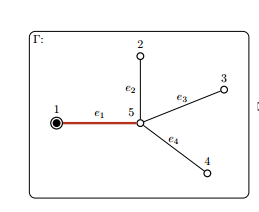
\includegraphics[width=0.7\linewidth]{fig1}
		\caption{Граф для конвертации из \cite{CorMgTapn}}
		\label{fig:fig1}
	\end{figure}
	Запустим программу для данного графа:
	\begin{figure}[h!]
		\centering
		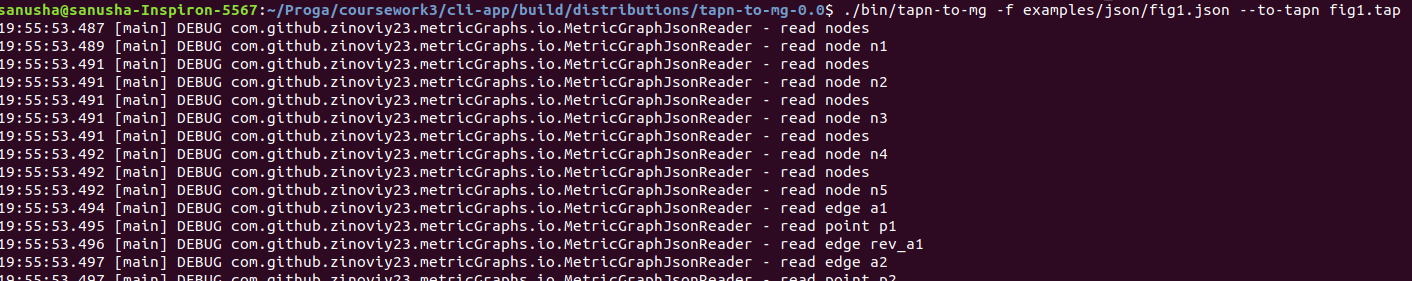
\includegraphics[width=0.7\linewidth]{run_fig1}
		\caption{Запуск конвертации}
		\label{fig:runfig1}
	\end{figure}
	
	Откроем результат в Tapaal\cite{tapaal}.
	
	\begin{figure}[h!]
		\centering
		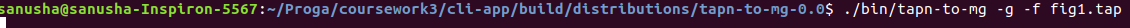
\includegraphics[width=0.7\linewidth]{run_tapaal}
		\caption{Открытие полученного файла в встроеном TAPAAL}
		\label{fig:runtapaal}
	\end{figure}
	
	\newpage
	\begin{figure}
		\centering
		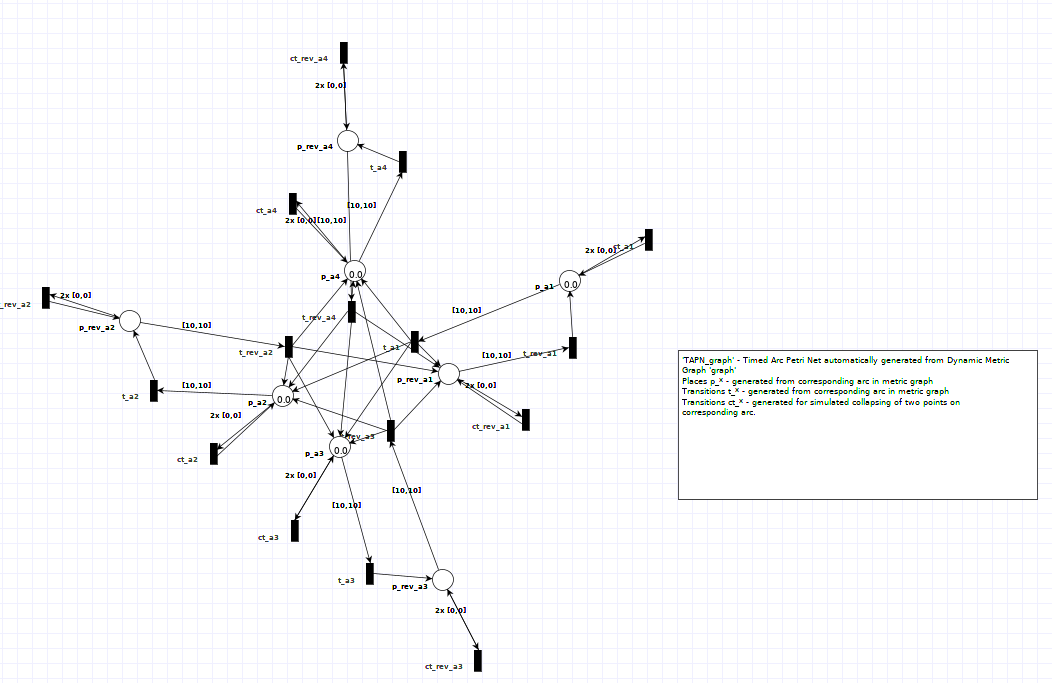
\includegraphics[width=0.9\linewidth]{result_tapn}
		\caption{Результат}
		\label{fig:resulttapn}
	\end{figure}
	Как видно, сеть сконвертирвалась правильно, так же к ней добавлено описание, чтобы понимать что происходит.

	\section{Конвертация из встроенной сети Петри в метрический граф}
	\begin{figure}[h!]
		\centering
		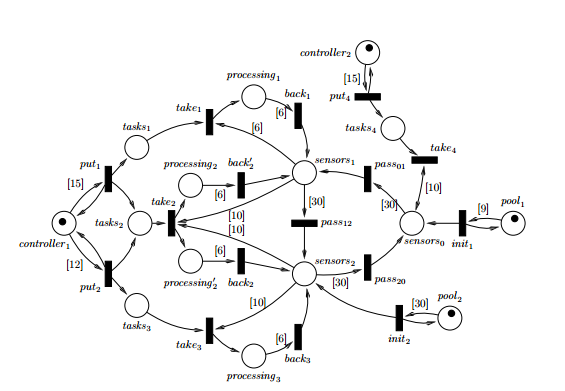
\includegraphics[width=0.7\linewidth]{fig4}
		\caption{Исходная временная сеть Петри\cite{CorMgTapn}}
		\label{fig:fig4}
	\end{figure}
	Запустим конвертацию в метрический граф в формате yed, для его визуализации:
	\begin{figure}[h!]
		\centering
		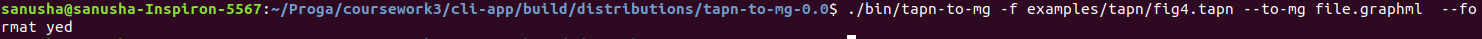
\includegraphics[width=0.7\linewidth]{run_to_mg}
		\caption{Запуск конвертации}
		\label{fig:runtomg}
	\end{figure}
	
	\newpage
	\begin{figure}[h!]
		\centering
		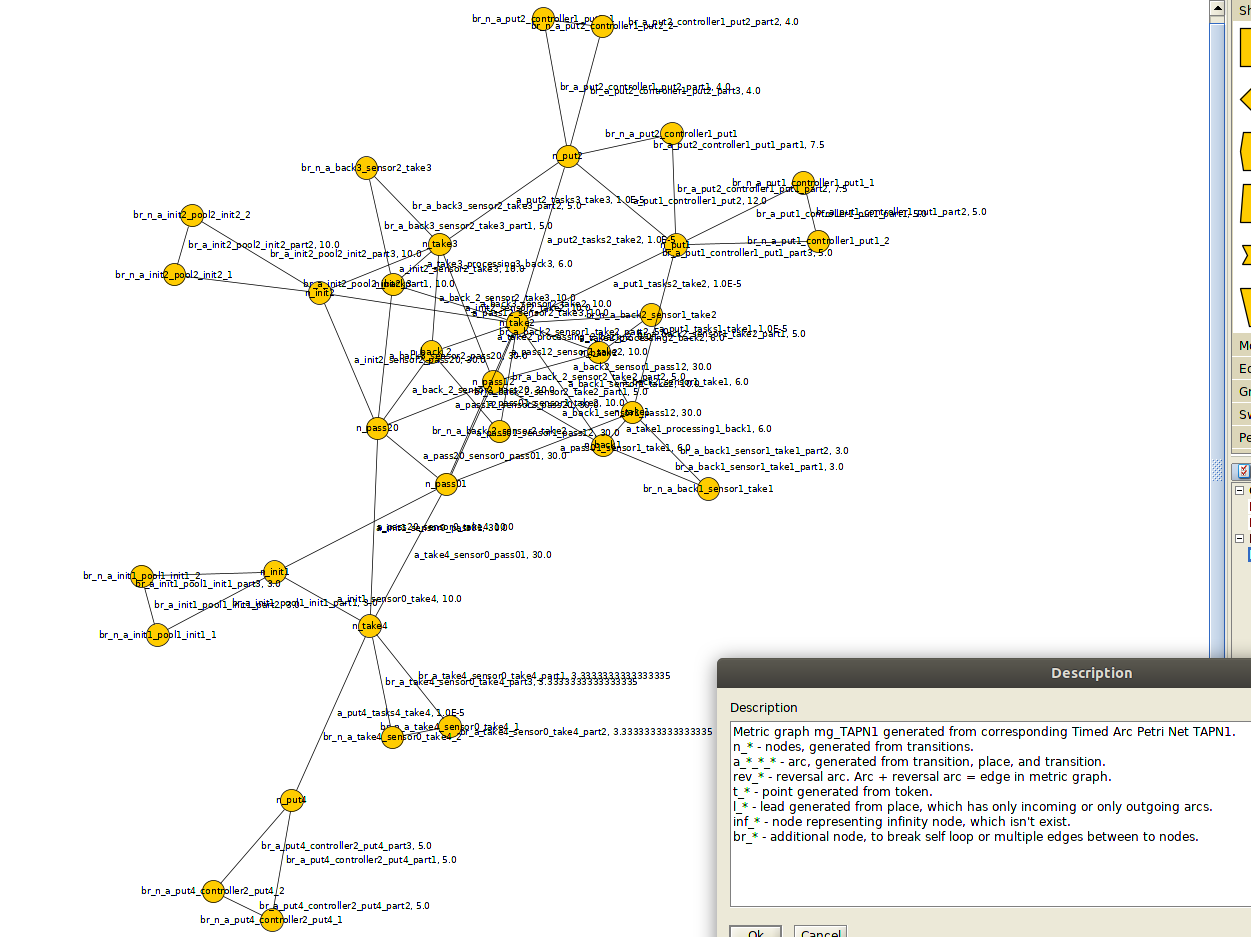
\includegraphics[width=0.9\linewidth]{yed}
		\caption{Полученный граф}
		\label{fig:yed}
	\end{figure}
	Откроем полученный файл в yEd Graph Editor\cite{yededitor}:
	Конвертация прошла успешно. Видно, что из-за кратных ребер появилось много дополнительных вершин, которые их ломают (br\_), так же видно, что обратные ребра не нарисованы, но представленны на графе.
	
	
	
	\newpage
	\bibliographystyle{utf8gost705u}  %% стилевой файл для оформления по ГОСТу
	\bibliography{../biblio}     %% имя библиографической базы (bib-файла)
	\addtocounter{section}{2}
	\addcontentsline{toc}{section}{Список используемых источников}
	
	\registrationList
\end{document}